%%%%%%%%%%%%%%%%%%%%%%%%%%%%%%%%%%%%%%%%%
%%            KHK-Vorlage              %%
%%                                     %%
%%         zur Erstellung eines        %%
%%        Buches mit pdflatex/latex    %%
%%                                     %%
%%               (Jan 2014)            %%
%%%%%%%%%%%%%%%%%%%%%%%%%%%%%%%%%%%%%%%%%

\documentclass[11pt,a4paper]{article}


%%%%%%%%%%%%%%%%%%%%%%%%%%%%
%%   Zusaetzliche Pakete  %%
%%%%%%%%%%%%%%%%%%%%%%%%%%%%

\usepackage[ngerman]{babel}	% neue deutsche Rechtschreibung
\usepackage[utf8]{inputenc}
%\usepackage{a4wide}
\usepackage{fancyhdr}
\usepackage{amsmath}
\usepackage{amsfonts}
\usepackage{caption}
%\usepackage{siunitx}
\usepackage{amssymb}
\usepackage{makeidx}
\usepackage{graphicx}		% Einbinden von Grafiken
%\usepackage{epstopdf}
\usepackage{lmodern}		% Schrift
\usepackage[T1]{fontenc}  	% access \textquotedbl
\usepackage{textcomp}     	% access \textquotesingle
\usepackage[]{natbib} 
\usepackage{booktabs}		% Tabellenlinien
\usepackage{rotating}		% Tabellen quer auf Seite
\usepackage{tensor}			% für Tensoren nützlich

% \usepackage{longtable}
% Tabellen über mehrere Seiten hinweg: 
% Multi-page Tables
% The longtable package defines an environment called longtable,
% which has a similar functionality as the tabular environment. 


% \usepackage{url}			% package url und hyperref haben ähnliche Funktionalität
%  Da es mit dem Paket hyperref und anderen Paketen zu Problemen kommen kann, sollte \usepackage{hyperref} der letzte Paketaufruf sein. Wird für DOI in Bibliographie benötigt

\usepackage[unicode=true,bookmarks=true,bookmarksnumbered=true,bookmarksopen=false, breaklinks=true,pdfborder={0 0 1},backref=false,colorlinks=true]{hyperref}

% Hinweis: \title{um was auch immer es geht}, \author{wer es auch immer 
% geschrieben hat} und  \date{wann auch immer das war} können vor 
% oder nach dem  Kommando \begin{document} stehen 
% Aber der \maketitle Befehl muß{} nach dem \begin{document} Kommando stehen! 

\title{Christoffelsymbole - einfach erklärt! \\
      Herleitung für den ART Workshop Erding}
\author{von Christophe und Karl-Heinz}
\date{\today}

% \date{\today} das heutige Datum  
% \date{25.12.00} oder ein bestimmtes Datum 
% \date{ } oder gar kein Datum


% Macros
% sehr gut: http://www.math.tamu.edu/~boas/courses/math696/gnuly-married.html

\newcommand{\christoffel}[3]{\ensuremath{\Gamma^{#1#2}_{#3}}}



%%%%%%%%%%%%%%%%%%%%%%%%%%%%
%%  Beginn des Dokuments  %%
%%%%%%%%%%%%%%%%%%%%%%%%%%%%


\begin{document}

\maketitle

\section{Konventionen und Vereinbarungen}

\begin{itemize}

\item SR = Spezielle Relativitätstheorie

\item ART = Allgemeine Relativitätstheorie

\item 
Zur Beschreibung eines Vektors kann man verschiedene Begriffe verwenden. Wir verwenden den Begriff "`Startpunkt"' für den Anfang, Ursprung oder Fußpunkt und den Begriff "`Endpunkt"' für die Spitze eines Vektors. 

\item 
Die Lichtgeschwindigkeit c kann zwar in den aus dem Alltag bekannten Einheiten $ [km/h] $ bzw. $ [km/s] $  angegeben werden. Dies führt jedoch zu unhandlichen Formeln. Aus diesem Grund wurde die Konvention eingeführt, die Lichtgeschwindigkeit $ [c = 1] $ zu setzen. 

\item
Lateinische Indizes, z. B. k, l oder m, werden verwendet, wenn drei Indexstufen \{0, 1, 2\} vorliegen.
Griechische Indizes, z. B. $ \mu $ oder $ \nu $ werden verwendet, wenn vier Indezstufen \{0, 1, 2, 3\} vorliegen.


\end{itemize}

\section{Einleitung}

Todo: Quelle ergänzen = Bertschinger, Introduction to Tensor Calculus for GR, MIT, 1999

Zum Verständnis der Allgemeinen Relativitätstheorie (ART) sind folgende Aspekte von besonderer Bedeutung. 

\begin{itemize}
	\item Raum-Zeit kann als vierdimensionaler Raum betrachtet werden. Durch den Einfluß der Gravitation ist das Raum-Zeit-Kontinuum "gekrümmt", d.h. im Gegensatz zur euklidschen Geometrie sind die Abstände zwischen den Koordinatenlinien nicht mehr "`äquidistant"'. Man spricht in diesem Zusammenhang davon, dass das Raum-Zeit-Kontinuum "`gekrümmt"' ist. Als Folge davon benötigt man zum Beschreiben physikalischer Zusammenhänge eine mathematische Form, die es erlaubt diese Gesetzmässigkeiten unabhängig von Koordinatensystemen zu beschreiben. Genau für diese Aufgabe eignen sich Tensoren sehr gut, so dass es erforderlich ist, die Tensornotation und Tensoralgebra zu lernen, wenn man sich mit ART beschäftigen möchte.
	
	\item Da man davon ausgeht, dass Raum-Zeit differenzierbar ist, was übrigens durch den Ausdruck Raum-Zeit-Kontinuum ausgedrückt wird, kann man für infinitesimal kleine Änderung der Raum-Zeit-Position lokal flache Koordinatensysteme formulieren, in denen dann näherungsweise wie in euklidschen, also flachen Räumen gerechnet werden kann.
\end{itemize}

Betrachtet man die gekrümmte Raum-Zeit der Allgemeinen Relativitätstheorie im Gegensatz zur speziellen Relativitätstheorie, bei der der dreidimensionale Raum nach euklidschen Kriterien beschrieben wird während die Zeit absolut ist, dann ändert sich die Interpretation der Bahnkurve von Partikeln wie folgt.

Nach der Newtonschen Interpretation wirkt die Gravitation auf Partikel im Raum und bewirkt eine Beschleunigung, die ihre Bahnkurve beeinflußt. Aus dem Gesichtspunkt der ART verursacht die Gravitation keine Beschleunigung der Partikel, sondern führt zu einer Krümmung von Raum-Zeit. Die Bahnkurve eines Partikels wird dann nicht unter dem Aspekt des Wirkens einer externen Kraft betrachtet. Solange keine zusätzlichen externen Kräfte wirken, bewegen sich die Partikel entlang der kürzesten Verbindung von zwei Punkten. Diese Verbindung wird als Geodäte bezeichnet. Aus dem Gesichtspunkt der SR mag diese Bahnkurve "gekrümmt" erscheinen. Im Bezugssystem der ART hingegen ist diese Bahnkurve eine Geodäte. 

Diese Zusammenhänge werden mit Hilfe der Einsteinschen Feldgleichungen beschrieben.



\section{Koordinatensysteme}

Mit Hilfe von Koordinaten kann man geometrische Probleme algebraisch lösen, d. h. man kann mit geometrischen Objekten "`rechnen"'. 

Ein Koordinatensystem verbindet Punkte im Raum mit einer Menge von Zahlen. Es gibt zahlreiche Möglichkeiten, ein Koordinatensystem zu wählen. Beispiele sind das klassische karthesische Koordinatensystem, Polarkoordinaten, Zylinderkoordinaten oder sphärische Koordinaten. Die Fragestellung entscheidet, welches Koordinatensystem man verwendet. Man kann zwar prinzipiell mit allen Koordinatensystemen arbeiten, manche Problem lassen sich aber sehr elegant lösen, wenn man das passende Koordinatensystem auswählt. Möchte man z. B. die Oberfläche der Erde vermessen, bietet sich ein sphärisches Koordinatensystem an. Würde man alternativ ein karthesisches Koordinatensystem verwenden, wäre die Beschreibung der Erdoberfläche zwar ebenso möglich, die Form der Koordinaten wäre aber ungleich komplizierter.

\subsection{Vektoren}
\subsection{ Differentialform vom Grad 1, kurz 1-Form (engl. one-form)}
\subsection{Tensoren}


KHK todo:

Beschreiben von verschiedenen Koordinatensystemen wie z. B. bei Grinfeld ab Kapitel 3.6.

\subsection{Karthesische Koordinaten}

\subsection{Affine Koordinaten}

\subsection{Polarkoordinaten}

\subsection{Zylinderkoordinaten}

\subsection{Sphärische Koordinaten}

\section{Umrechnung zwischen verschiedenen Koordinatensystemen}

KHK todo: Grinfeld Kapitel 4

\section{Grundlagen der Tensornotation}

KHK todo: Grinfeld Kapitel 4.9 und andere Autoren zur Ergänzung

\section{Tensorbeschreibung des Euklidschen Raumes}

KHK todo: Grinfeld Kapitel 5 aber auch schon Kapitel 6 in Auszügen
 
\subsection{Koordinatenbasis}

\subsection{Metrischer Tensor}

\section{Kovariante Ableitung}

KHK todo: Grinfeld Kapitel 8

Bitte prüfen - welche Gliederung hat Susskind gewählt. Gliederung evtl. entsprechend anpassen.

Evtl. ist es sinnvoll, die kovariante Ableitung als subsection der Tensorbeschreibung zu gliedern.

\section{Christoffelsymbole}

KHK todo: Grindfeld Kapitel 5.14 und andere Autoren

% Packet graphix einbinden
% Grafik in Inkscape als eps abspeichern
% Hier: ohne Rahmen um Grafik
% Achtung: Immer zuerst \caption und danach erst \label! 
% Wird dies nicht beachtet, so stimmen die Verweise auf die Bilder nicht mit den Bildnummern überein.
% Verweis auf Bild im Text: Bild~\ref{pic:DasBild} zeigt ...
% Anmerkung: Die Tilde sorgt dafür, dass an dieser Stelle nicht umbrochen wird und dass der Abstand konstant bleibt.


Im Folgenden werden die Christoffelsymbole und ihre Bedeutung anhand eines einfachen Beispiels dargestellt. Wir wollen sehen welche Rolle ein Bezugssystem bzw.  Koordinaten spielt, dazu arbeiten wir zunächst so weit es geht ohne Bezugssystem bzw. Koordinaten. Anschließend führen wir am Beispiel eines "`lokalen Bezugssystems"' Koordinaten ein. Wie wir das Bezugssystem auswählen wird zunächst willkürlich erscheinen. Wir wollen nur die Symbole am Beispiel von Polarkoordinaten im "flachen Raum" darstellen, ohne komplett zu erklären, wofür sie gut sind.

Wir gehen von zwei willkürlich gewählten Vektoren aus (Abb. \ref{fig:Vektoren-ohne-alles}). Allein die Tatsache, dass wir Vektoren betrachten, ist ein Hinweis darauf, dass wir im flachen Raum (euklidischer Raum) arbeiten. 

\bigskip
Einschub KH: bitte diesen "`Hinweis"' kurz erklären. Uns ist es inzwischen bewußt, aber für zukünftige Kurse wäre es hilfreich, dies zu erläutern. Versuch von mir: 

Nach klassischem Schulwissen versteht man unter einem Vektor die Menge aller Pfeile mit gleicher Richtung und gleichem Betrag. Man kann sich das auch so vorstellen, dass man einen Vektor im Raum entlang einer geschlossenen Kurve verschieben kann und der Vektor hat noch die selbst Länge und Richtung wie zuvor, wenn er wieder am Ausgangspunkt ankommt. Dies gilt nicht für gekrümmt Räume. 

Einschub Ende
\bigskip

Es ist wichtig zu verstehen, dass die zwei Vektoren und wie sie zueinander stehen, unabhängig von irgendeinem Bezugssystem bzw. Koordinatensystem sind. 

\begin{figure}
  \centering
  \mbox{
    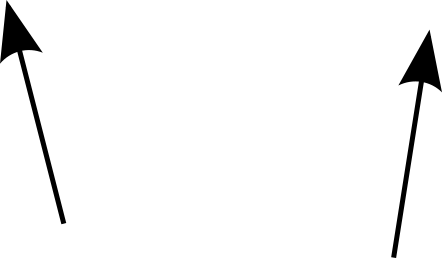
\includegraphics[width=4cm]{img/Christoffel-Zeichnung-1.png}
  }
    \captionsetup{singlelinecheck=off}
    \caption[.]{Wir gehen von zwei beliebigen Vektoren aus.
	% eine separate Zeile mit Mathe würde man so eingeben:
	%    
	%    \begin{displaymath}
	%        assoc\_meaning(\&actor(x) maintained(x,\nonumber <(dist\_from(y),1))
	%    \end{displaymath} 
	}
    \label{fig:Vektoren-ohne-alles}
\end{figure}

Wenn wir die beiden Vektoren vergleichen wollen, können wir z.B. ihre Differenz bilden, also
\begin{align*}
	\Delta \overrightarrow{v} &=   \overrightarrow{v}_{(r,\theta)} - \overrightarrow{v}_{(r',\theta')}\\
\end{align*} 
Um diese Differenz zu bilden, kann man einen der beiden Vektor zum anderen verschieben und zwar so, dass sich die Startpunkte der beiden Vektoren berühren. Dies ist im flachen Raum z. B. durch geometrische Konstrukten mit Zirkel und Lineal einfach möglich. Die Differenz ist dann ein weiterer Vektor, der ebenfalls von Koordinaten völlig unabhängig existiert.

Wir führen jetzt ein Koordinatensystem ein. Das bedeutet, dass wir "`Zahlen"' mit geometrischen Objekten assoziieren wollen, damit wir mit diese Objekte rechnen können.

Als Koordinatensystem wählen wir ein Polarkoordinatensystem. Vom Ursprung des Polarkoordinatensystems zum Anfangpunkt der Vektoren wird je ein Ortsvektor eingezeichnet. Der Anfang eines Vektors hat meist eine physikalische Bedeutung, z.B. als Bezugspunkt für Kräfte oder die Geschwindigkeit eines Objekts. 

Die Anfangspunkte ("`Startpunkte"') der beiden Vektoren $ \overrightarrow{v}_{(r,\theta)} $ und $ \overrightarrow{v}_{(r',\theta')} $ in  Abb. \ref{fig:Vektoren-und-Ortsvektoren} sind als Funktion des Abstand vom Nullpunkt und des Winkels zu dem horizontalen Strahl des hier willkürlich gewählten Polarkoordinatensystems eingezeichnet.

\begin{figure}
  \centering
  \mbox{
    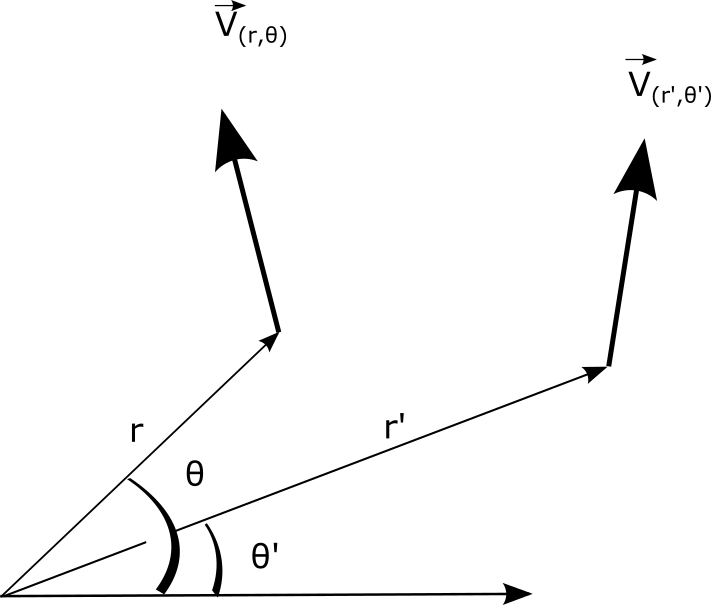
\includegraphics[width=8cm]{img/Christoffel-Ortsvektoren.png}
  }
    \captionsetup{singlelinecheck=off}
    \caption[.]{Diese beiden Vektoren können wir in Abhängigkeit von r und $ \theta $ und r' und $ \theta$' ausdrücken: $ \overrightarrow{v}_{(r,\theta)} $ und $ \overrightarrow{v}_{(r',\theta')} $ 
    
	% eine separate Zeile mit Mathe würde man so eingeben:
	%    
	%    \begin{displaymath}
	%        assoc\_meaning(\&actor(x) maintained(x,\nonumber <(dist\_from(y),1))
	%    \end{displaymath} 
	}
    \label{fig:Vektoren-und-Ortsvektoren}
\end{figure}

Als Nächstes wollen wir die Vektor-Endpunkte mit Zahlen versehen. Die Endpunkte sind zunächst auch einfach nur Punkte, die man ebenfalls im gewählten Polarkoordinatensystem beschreiben könnte. Dies ist jedoch nicht der eleganteste Ansatz:
\begin{itemize}
\item Die Vektorendpunkte existieren meistens NICHT in ursprüngliche Raum, also es ist nicht viel zu erwarten wenn wir so tun.
\item Diese Verfahren kann man sicher nicht in gekrümmte Raum verallgemeinern, da Vektoren dort nicht ohne weiteres existieren.
\end{itemize}

Wir legen ein neue, diesmal lokale Koordinatenbasen in die Startpunkte der beiden Vektoren. Wir könnten jeweils ein beliebige Basis auswählen, aber es ist ratsam die Basis irgendwie von den Koordinatensystem abzuleiten, damit kann man quasi automatisch die Basis an jeden Punkt berechnen. Um genau zu sein reicht das Koordinatensystem nicht aus, die "`Geometrie"' der Raum (in unsere Fall flach) muss irgendwie einbezogen werden. Wir werden sehen wie es geschieht. 

Auch wenn wir von den Koordinatensystem ausgehen, gibt es trotzdem unendlich viele Freiheiten wie wir das machen. Wir wählen folgende Methode aus:
\begin{itemize}
\item die Richtung der Vektor wird entlang die Änderung von jeder Koordinaten gewählt. D.h., dass wir für eine Vektor $r$ konstant halten und wir lassen $\theta$ ein bisschen variieren. wenn die Variation klein ist, definiert es eine Richtung. Wir machen dann dasselbe mit dem andere Koordinate
\item die Länge wird proportional zu den metrische Änderung die beim Koordinateänderungen produziert werden. D.h, wenn wir $\theta$ um $\delta\theta$ ändern, der Punkt transportiert sich um $r\delta\theta$. Beim $r$, ist es einfach $\delta r$.
\end{itemize}
Diese Art von Basis "`arbeitet"' sehr schön mit dem Tensor Formalismus, da, wir iwr werden sehen, bei Basiswechseln die Komponenten "`ko"'- und "`kontravarianten"' Eigenschaften haben.

\begin{figure}
  \centering
  \mbox{
    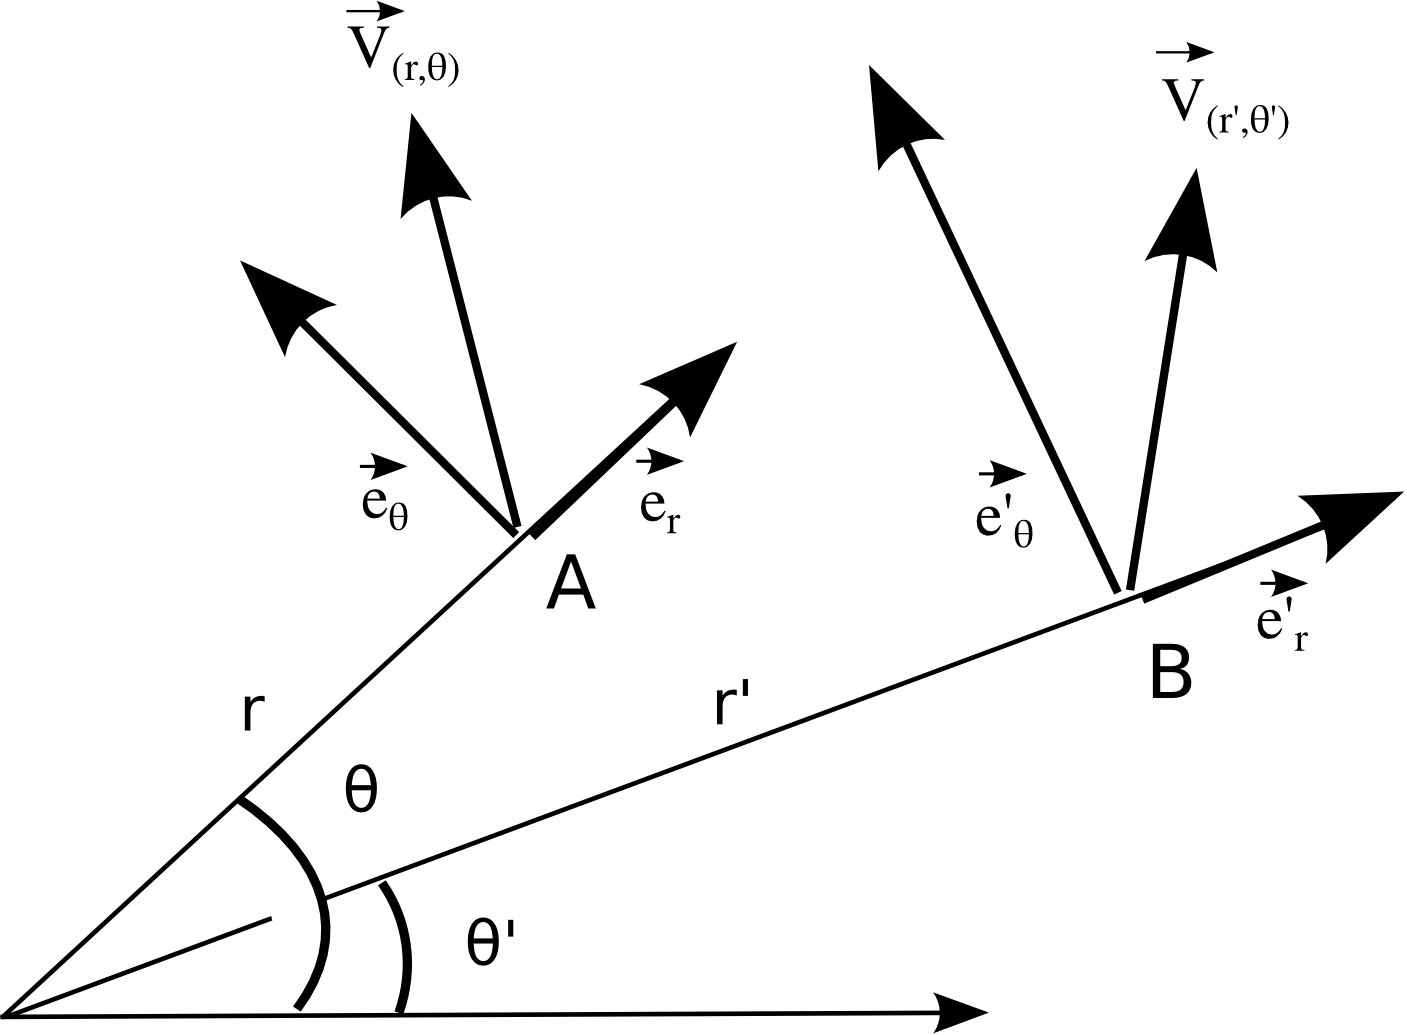
\includegraphics[width=8cm]{img/Christoffel-Zeichnung.png}
  }
    \captionsetup{singlelinecheck=off}
    \caption[.]{Jedem der beiden Vektoren $ \overrightarrow{v}_{(r,\theta)} $ und $ \overrightarrow{v}_{(r',\theta')} $ kann man eine eigene Basis zuordnen: A mit den Basisvektoren $ \overrightarrow{e}_{r} $ und $ \overrightarrow{e}_{\theta} $, und B mit den Basisvektoren $ \overrightarrow{e}_{r'} $ und $ \overrightarrow{e}_{\theta'} $. Wichtig: die Länge von alle $\overrightarrow{e}_{r}$ ist konstant und beträgt $1$, dagegen die Längen von $ \overrightarrow{e}_{\theta} $ ist $|r|$. Der Grund ist, dass wir ein Basis wollen die an die Koordinaten {\it angepasst} ist. Da ein Änderung von $\delta\theta$ auf ein Punkt bewirkt ein Streckenänderung mit dem Länge $r\delta\theta$ (Strahlensatz), ist unsere Wahl damit konsistent.
    
	% eine separate Zeile mit Mathe würde man so eingeben:
	%    
	%    \begin{displaymath}
	%        assoc\_meaning(\&actor(x) maintained(x,\nonumber <(dist\_from(y),1))
	%    \end{displaymath} 
	}
    \label{fig:Vektoren-und-Basen}
\end{figure}

Sobald die Basen A und B gewählt wurden, kann man $ \overrightarrow{v}_{(r,\theta)} $ und $ \overrightarrow{v}_{(r',\theta')} $ auch mit Hilfe der lokalen Basen A und B ausdrücken.

\begin{align*}
	\overrightarrow{v}_{(r,\theta)} &= v^{\theta} \overrightarrow{e}_{\theta} + 
	                                   v^{r} \overrightarrow{e}_{r}                \\
	\overrightarrow{v}_{(r',\theta')} &= v^{\theta'} \overrightarrow{e}_{\theta'} + 
	                                     v^{r'} \overrightarrow{e}_{r'}
\end{align*} 
 
\begin{align*}
	\Delta v &=   \overrightarrow{v}_{(r,\theta)} - \overrightarrow{v}_{(r',\theta')}\\
			&=  v^{\theta} \overrightarrow{e}_{\theta} + v^{r} \overrightarrow{e}_{r}  - v^{\theta'} \overrightarrow{e}_{\theta'} - v^{r'} \overrightarrow{e}_{r'}   \\
\end{align*} 

Jetzt wollen wir die Vektoren A und B vergleichen. Damit werden wir A zu B transportieren. Wir machen es in 2 Schritten:
\begin{itemize}
\item zu nächst lassen wir $r$ konstant und ändern wir nur $\theta$
\item dann lassen wir $\theta$ konstant und ändern wir $r$
\end{itemize}
Wenn wir so machen, können wir später den klassische Analysis Formalismus benutzen (also multidimensionale Differentielle,...)

\begin{figure}
  \centering
  \mbox{
    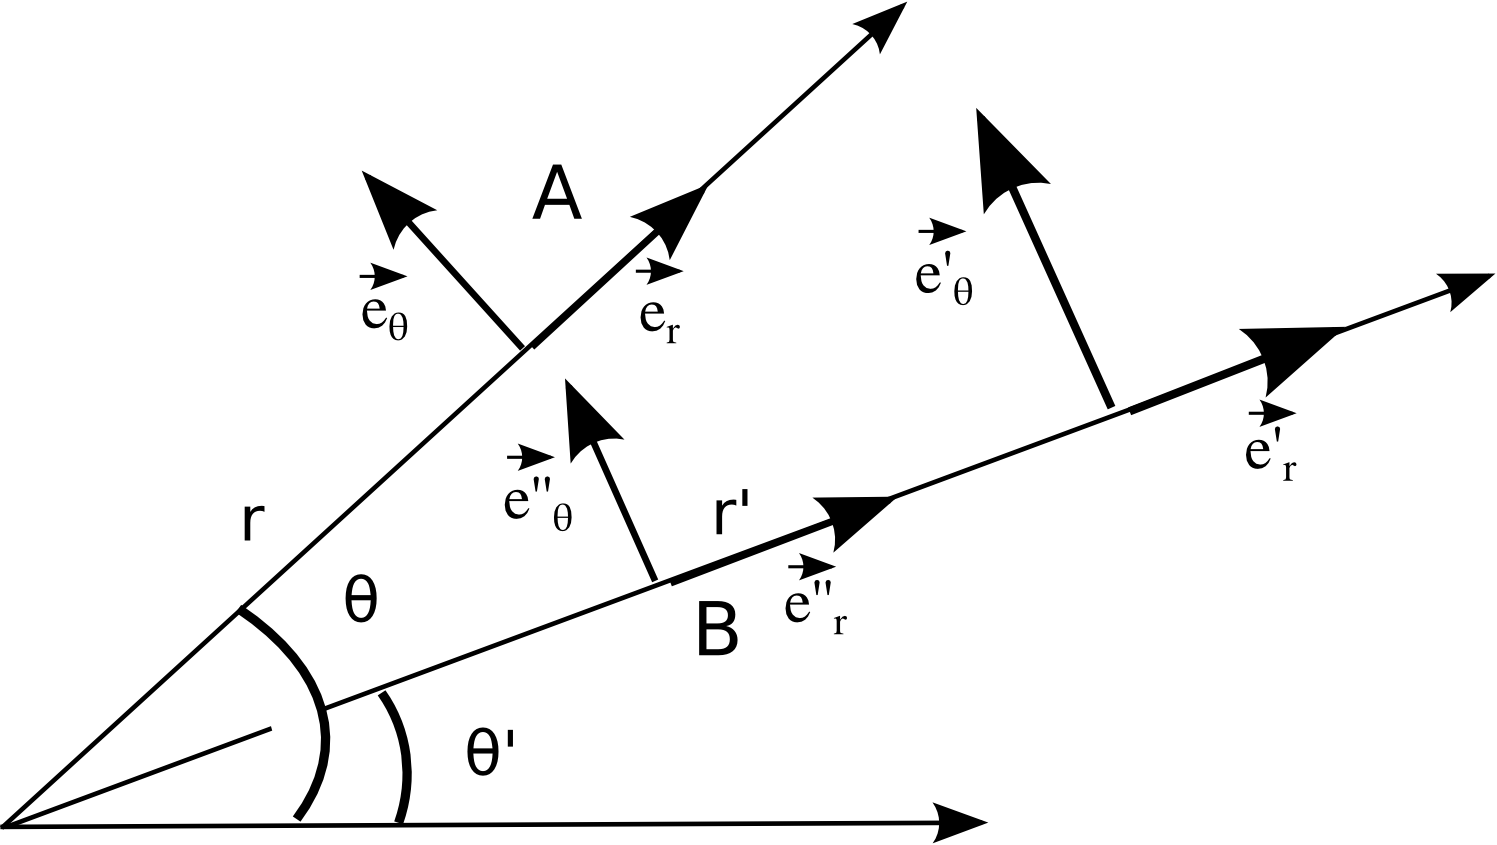
\includegraphics[width=8cm]{img/Christoffel-Zeichnung -Verschiebung theta.png}
  }
    \captionsetup{singlelinecheck=off}
    \label{fig:Verschiebung Teil 1}
\end{figure}


Den Übergang von $ \overrightarrow{v}_{(r,\theta)} $ zu $ \overrightarrow{v}_{(r',\theta')} $ kann man mit Hilfe eines kleinen Verschiebevektors ausdrücken der ebenfalls eine lokale Basis bekommt. Die Komponenten und die Basis des Verschiebevektors werden mit $\delta$ gekennzeichnet. Durch Ausmultiplizieren und Zusammenfassen erhält man:

\begin{align*}
	&= v^{\theta} \overrightarrow{e}_{\theta} + v^{r} \overrightarrow{e}_{r} - (v^{\theta} + \delta v^{\theta})(\overrightarrow{e}_{\theta} + \delta\overrightarrow{e}_{\theta}) - (v^{r} + \delta v^{r})(\overrightarrow{e}_{r} + \delta\overrightarrow{e}_{r}) \\
	\Delta v &= \delta v^{\theta} \overrightarrow{e}_{\theta} - 
	   v^{\theta} \delta \overrightarrow{e}_{\theta} + 
	   \delta v^{r} \overrightarrow{e}_{r} - 
	   v^{r} \delta \overrightarrow{e}_{r}						\\
	&= - (\delta v^{\theta} \overrightarrow{e}_{\theta} + 
	    \delta v^{r} \overrightarrow{e}_{r} ) - 
	   ( v^{\theta} \delta\overrightarrow{e}_{\theta} + 
	     v^{r} \delta\overrightarrow{e}_{r} )
\end{align*} 




\begin{figure}
  \centering
  \mbox{
    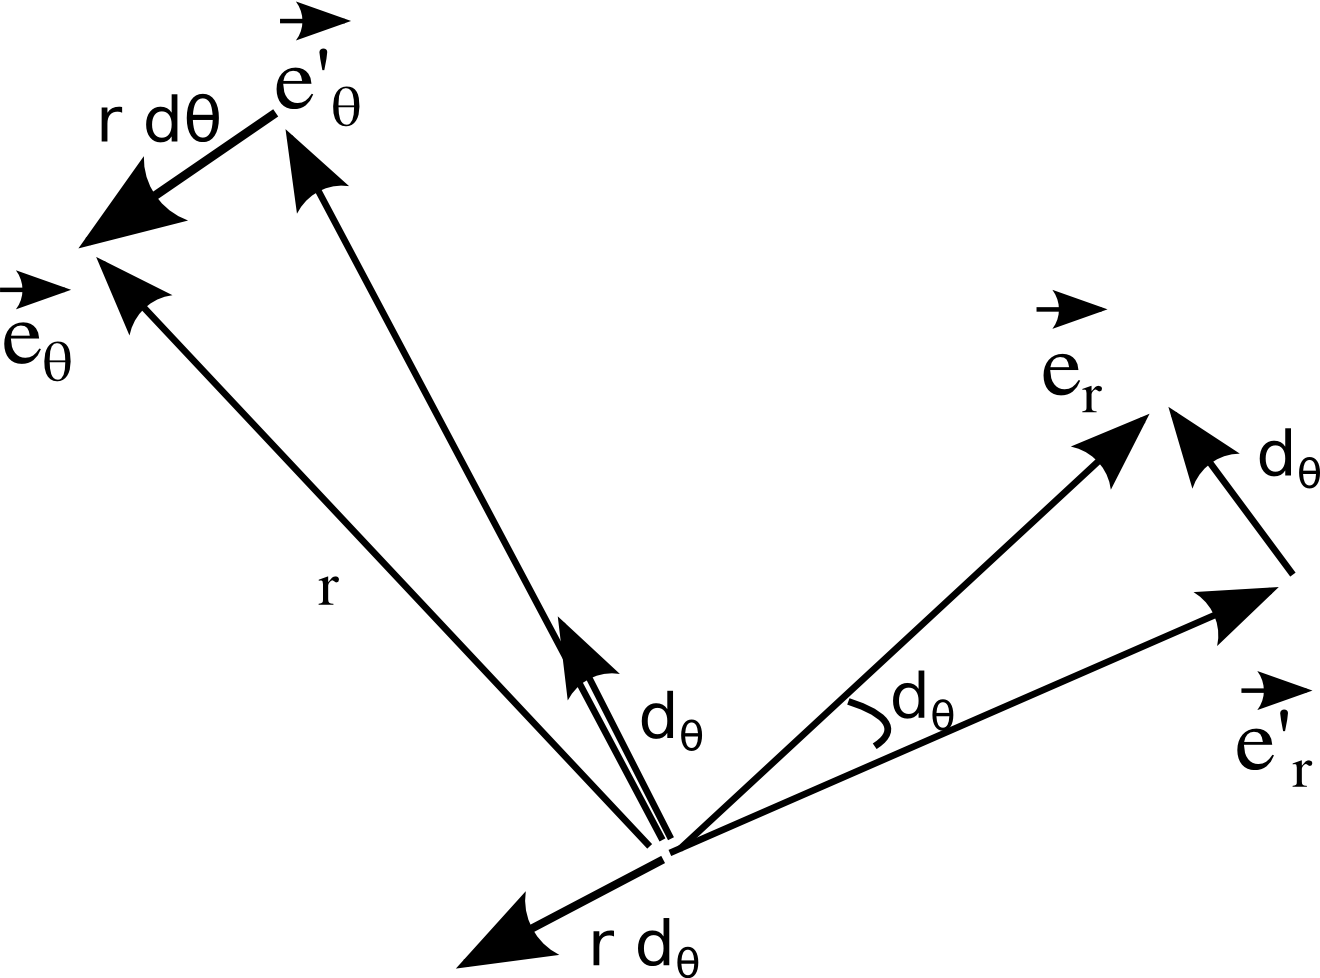
\includegraphics[width=8cm]{img/Christoffel-Zeichnung-phi.png}
  }
    \captionsetup{singlelinecheck=off}
    \caption[.]{wir haben eine Basis zu den andere parallel transportiert um die besser vergleichen zu können. die Änderungen der Basis Vektoren sind als "r d$\theta$ und $\theta$  angegeben. Da $\overrightarrow{e}_{\theta} $. $r$ mal länger ist als $\overrightarrow{e}_{r}$ muss man in der Koeffizient ein Korrekturfaktor einfügen wenn man die Änderung auf die Basisvektoren expandieren wollen. Ergebnis ist dann: $\overrightarrow{\delta\theta}= \overrightarrow{\delta e}_{r}=\frac{1}{r}\overrightarrow{e}_{\theta}$ und $\overrightarrow{r \delta\theta}= \overrightarrow{\delta e}_{\theta}=-r\overrightarrow{e}_{r}$
    
	% eine separate Zeile mit Mathe würde man so eingeben:
	%    
	%    \begin{displaymath}
	%        assoc\_meaning(\&actor(x) maintained(x,\nonumber <(dist\_from(y),1))
	%    \end{displaymath} 
	}
    \label{fig:nur Delta Phi}
\end{figure}
 
\end{document}
